\pdfoutput=1 % Tell arXiv to use pdfLaTeX. Do not remove this line.

\documentclass[11pt]{article}

% Remove the "review" option to generate the final version.
\usepackage[review]{emnlp2021}
% \usepackage{emnlp2021}
\usepackage{times}
\usepackage{xspace}
\usepackage{latexsym}
\usepackage[T1]{fontenc}
\usepackage[utf8]{inputenc}
\usepackage{microtype}
\usepackage{graphicx}
\usepackage{relsize}
\usepackage{tabularx}
\usepackage{booktabs}
\usepackage{amsmath}
\usepackage{amssymb}
\usepackage{subcaption}
\usepackage{float}
\usepackage{csquotes}
\graphicspath{{figures/}}
\newcommand{\ArgKP}{\mbox{ArgKP}\xspace}
\newcommand{\ArgQ}{\mbox{IBM-ArgQ-Rank-30kArgs}\xspace}
\newcommand{\Bert}{\textsc{Bert}\xspace}
\newcommand{\BertBase}{\Bert-Base\xspace}
\newcommand{\BertLarge}{\Bert-Large\xspace}
\newcommand{\Roberta}{\mbox{Ro\textsc{Bert}a}\xspace}
\newcommand{\RobertaBase}{\Roberta-Base\xspace}
\newcommand{\Albert}{\textsc{Albert}\xspace}

% Draft editing helpers. Remove 
\newcommand{\todocite}{{\smaller\color{red}[CITE]}\xspace}
\newcommand{\todo}[1]{{\smaller\color{red}[#1]}}

\title{%
  Modern Talking in Key Point Analysis: \\
  Key Point Matching using Pretrained Encoders%
}
\author{%
  Jan Heinrich Reimer \and Thi Kim Hanh Luu \and Max Henze \and Yamen Ajjour \\
  Martin Luther University Halle-Wittenberg, Germany \\ 
  \texttt{\{%
  \href{mailto:jan.reimer@student.uni-halle.de}{\textcolor{black}{jan.reimer}},%
  \href{mailto:thi.luu@student.uni-halle.de}{\textcolor{black}{thi.luu}},%
  \href{mailto:max.henze@student.uni-halle.de}{\textcolor{black}{max.henze}}%
  \}@student.uni-halle.de} \\ 
  \texttt{\href{mailto:yamen.ajjour@informatik.uni-halle.de}{\textcolor{black}{yamen.ajjour@informatik.uni-halle.de}}}%
}

\begin{document}

\maketitle

\begin{abstract}
  We contribute to the ArgMining~2021 shared task on Quantitative Summarization and Key Point Analysis with two approaches 
for argument key point matching.
For key point matching the task is to decide if a short key point matches the content of an argument with the same topic 
and stance towards the topic.
We approach this task in two ways:
First, we develop a simple rule-based baseline matcher by computing token overlap after removing stop words, stemming, 
and adding synonyms/antonyms.
Second, we fine-tune pretrained \Bert and \Roberta language models as a regression classifier for only a single epoch.
We manually examine errors of our proposed matcher models and find that long arguments are harder to classify. Our fine-tuned \RobertaBase model achieves a mean average precision score of~0.913, the best score for strict labels of all participating teams.

\end{abstract}

\section{Introduction}\label{introduction}

Arguments influence our decisions in many places of our cultural life~\cite{Bar-HaimEFKLS2020}.
But with the increasingly larger amount of information found on the Web\footnote{\url{https://internetlivestats.com/}} and more efficient argument mining, people often need to summarize arguments~\cite{LawrenceR2019,Bar-HaimEFKLS2020}.
\citet{Bar-HaimEFKLS2020} see matching key points to arguments as an intermediate step towards automatically generating argumentative summaries~(Section~\ref{related-work}).
The ArgMining~2021 shared task on Quantitative Summarization and Key Point Analysis is the first task on key point matching, hence taking a step towards summarizing arguments~\todocite.
Different approaches of matching argument key point pairs, here called matchers, should be proposed and discussed.
\todo{Cite the task overview paper once the citation is announced.}
The shared task organizers therefore introduce a customized mean average precision evaluation metric and publish the ArgKP benchmark dataset~(Section~\ref{data}) to compare matchers~\todocite~\cite{Bar-HaimEFKLS2020}.

Large, pretrained language models like \Bert or \Roberta are frequently used to tackle various natural language processing tasks~\cite{DevlinCLT2019,LiuOGDJCLLZS2019}. \todo{Cite general, comparative paper, maybe GLUE.}
Because of their extensive pretraining, often fine-tuning those language models with even a small task-specific dataset can achieve state-of-the-art performance~\todocite.
As the ArgKP dataset~\cite{Bar-HaimEFKLS2020} used in the ArgMining~2021 shared task on Quantitative Summarization is relatively small~(24\,000 labelled matches), we decide to fine-tune \Bert and \Roberta language models rather than train a neural classifier from scratch~(Section~\ref{approach}).
Our fine-tuned \RobertaBase model achieves a mean average precision score of up to~0.967 and ranks second in the shared task's leaderboard~(Section~\ref{results}).

Contrasting the deep learning fine-tuning approach, we discus a simple rule-based baseline matcher that compares preprocessed terms of each argument to the terms of each key point~(Section~\ref{approach}). For the baseline, we compute term overlap similar to the Jaccard coefficient~\cite{Jaccard1902} after removing stop words, adding synonyms and antonyms, and stemming the tokens from both argument and key point using the NLTK~toolkit~\cite{BirdL2004}.
\section{Related Work}\label{related-work}

\subsection{Key Point Analysis}
Given the first track of the shared task analyzing key points is crucial. In their work \cite{Bar-HaimEFKLS2020} 
Bar-Haim et al. propose an approach for summarising large argument collections to small sets of key points. Thus
covering a sufficient amount of all arguments. They show that domain experts can very quickly
create pro and con key points, which are able to "capture the gist" of the arguments on the given topic. All this
without being exposed to the arguments themself. Furthermore they develop the large-scale dataset ArgKP
which is the foundation of this shared task. 
In a later work \cite{Bar-HaimKEFLS2020} Bar-Haim et al. construct an automatic method for key point 
extraction which can compete with key points created by human domain experts. The method consists of two aspects. 
Assuming that the key points can be found among the given comments 
they first select short, high quality comments as key point candidates an then select the candidate with the highest
data coverage. Using the HuggingFace transformer framework they fine-tune four different models from which 
ALBERT \cite{lan2019albert} has the best F1 score with $0.809$ but RoBERTa \cite{LiuOGDJCLLZS2019} (F1 score of 
$0.773$) is chosen for key point extraction since it has a 6 times faster inference time. 
In the paper \cite{egan2016summarising}, Egan et al. propose a summarising for informal arguments such as they
occure in online political debates. By extracting verbs and their syntactic arguments they retrieve points which
can make key content accessible. By grouping these points they propose to create discussion summaries.

\subsection{Argument Clustering}
Argument Clustering is a mighty tool that enables algorithms to assign multiple arguments, which adress a similar
key message to a given topic. In the paper \cite{reimers2019classification}, Reimers et al. make use of 
"contextualize word embeddings to classify and cluster topic-dependet arguments". Having performed argument
classification they then compute similar and dissimilar pairs of arguments. Two approaches one with clustering
and one without are being used. 
Clustering arguments is achieved by usage of agglomerative hierarchical clustering \cite{day1984efficient}. 
Without clustering a fine-tuned BERT-base-uncased model reached a F1 mean score for similar and dissimilar
arguments of $0.7401$. 
Agglomerative hierarchical clustering being a strict partitioning algorithm, results for clustering perform
worse by up to 7.64pp (Bert-large F1 mean score: $0.7135$). Hence they conclude that "strict partitioning 
clustering methods introduce a new source of errors".
Another approach proposed in a paper \cite{ajjour2019modeling} by Ajjour et al. revolves around clustering 
arguments into so called frames which are "a set of arguments that focus on the same aspect". 
Thereby framing \cite{entman1993framing} only a specific information to present to the listeners and convince 
them of your stance.
They propose that an argument consists of two crucial parts. The topic and the frame.
Hence their approch splits into three steps: First, all arguments are clustered into $m$ topics. Second,
topical features are extracted from all arguments and therefore from its cluster. Third, the arguments are 
reclustered into $k$ non-overlapping frames. By utilizing k-means \cite{hartigan1979ak} for clustering
and \textit{Term Frequency-Inverse Document Frequency} (TF-IDF) for topic removal they achieved a F1 score of 
$0.28$.

\todo{Third paper: Argument Invention from First Principles (probably not crucial)}

\subsection{Stance Classification}
By knowing the stance of an argument it becomes nearly effortless for a human to classify it as pro or con 
to a given topic. 

\section{Data}\label{data}

The dataset used in this shared task is the \ArgKP dataset~\cite{Bar-HaimEFKLS2020} which consists of 24\,083 argument and key point pairs labeled as matching/non-matching. They all belong to one of 28 controversial topics, for example: \textquote{Assisted suicide should be a criminal offence}. Each of the pairs is also assigned a stance towards the topic. 

The split used for training has 5\,583~arguments belonging to 207 key points within 24~topics. This leaves the 
validation dataset with 932~arguments and 36~key points for 4~topics. The test dataset, which is used for evaluation of all submissions, contains 723~ arguments with 33~ key points. There are 3~ topics given in the test dataset.

\subsection{Characteristics}
\begin{table*}
    \caption{Examples of \todo{matching} argument key point pairs from the \ArgKP dataset~\cite{Bar-HaimEFKLS2020}}
    \label{examples}
    \begin{tabularx}{\linewidth}{lXp{4.3cm}c}
      \toprule
      \textbf{\#} & \textbf{Argument} & \textbf{Key point} \\
      \midrule
      A & % from training set, match
      child \textcolor{violet}{actors} can be overworked and they can miss out on their education. & % arg_13_153
      Being a \textcolor{violet}{performer} harms the child's education \\ % kp_13_5
      B & % from training set, match
      as long as nuclear weapons exist, the entire world has to worry about \textcolor{violet}{nations} deciding to fire them at another or \textcolor{violet}{terrorists} getting hold of them and causing disaster & % arg_17_91	
      Nuclear weapons can fall into the \textcolor{violet}{wrong hands} \\ % kp_17_1
      C & % from training set, not labelled
      `people reach their limit when it comes to their quality of life and should be able to end their \textcolor{violet}{suffering}. this can be done with little or no \textcolor{violet}{suffering} by \textcolor{teal}{assistance} and the person is able to say good bye. & % arg_0_0
      \textcolor{teal}{Assisted} suicide reduces \textcolor{violet}{suffering} \\ % kp_0_1
      \bottomrule
    \end{tabularx}
  \end{table*}


When analyzing the data, we realize that matched and unmatched key points of a given argument contain a certain proportion of the same words. 
Many of these words belong to the set of stop words, such as \textquote{as}, \textquote{for} and \textquote{not}.
They are also a part of the most common words from whole training set.
These words are uninformative for our prediction process, so that we remove stop words from our data during pre-processing. 
Furthermore, the important words from the argument are repeated with different tenses and parts of speech in key points, for example: \textquote{legalize}, \textquote{legalized}, \textquote{legalizing}, \textquote{legal}. 
To achieve an unambiguous spelling, such words are normalized with a stemming method in our approach. 
%This conversion to the word root reduces the size of the vocabulary or the dimensions of the text input.

In Table \ref{examples} we show examples of arguments key point pairs from the \ArgKP dataset \cite{Bar-HaimEFKLS2020}. 
We identify followed major difficulties in matching key points to arguments: semantically similar words and meaning understanding.
In the example pair~A from Table~\ref{examples}, the key point can be matched with its argument. Both sentences were written about children actors and their education. The word \textquote{actors} is not explicitly used in the key point but is semantically similar to the word \textquote{performer}. 
This poses a challenge for us to design our approach in such a way that it knows the different written words with the same meaning. 
A simple method we use is to apply the well-known lexical database WordNet for our baseline, to find the synonyms and antonyms \cite{Miller1995}.
It is recognized that the meaning of sentences understanding can be a challenge for the task. 
In the example~B from Table~\ref{examples}, the argument and the key point were expressed differently. 
We have in the key point these words \textquote{wrong hands} as figurative meaning of \textquote{nations} and \textquote{terrorists} from the argument. 
%There are two negations \textquote{not fair to not allow} and additionally a restriction with \textquote{as long as} for the main clause before used in the argument. 
To predict if the key point is aligned with the argument, we need to understand their meanings with different meaning arts and compare them. 
To better deal with this problem, we use two well-known language models in our second approach~(Section~\ref{approach}).
\section{Approach}\label{approach}

To match key points to arguments, we propose two different approaches.
First, we shortly discuss a simple yet effective baseline measuring term overlap between key points and arguments.
Second, to improve upon the simple baseline, we introduce a fine-tuning approach using \Bert~\todocite and \Roberta~\todocite pretrained language models. We use both language models in standard configuration with only minor changes highlighted below.

\subsection{Baseline}

We start with a very simple baseline. Therefore choosing a Term Overlap baseline with preprocessed terms. 
Generally it can be assumed, that key-points are summarizing ideas of all associated arguments. We therefore came up with the idea
that certain key-words, contained in a lot of arguments, are also very likely to be present in the associated key-point. This makes 
sense with our intuition, because rather than using completly new words for summarization of arguments, a human would 
rather reuse certain important words, which have been already found in the arguments.\\
\todo{Maybe this example fits better into the data section?}
For example, the following argument exists in the \ArgKP dataset:\\
\textit{People reach their limit when it comes to 
their quality of life and should be able to end their {\color{blue} suffering}. This can be done with little 
or no {\color{blue} suffering} by {\color{orange} assistance} and the person is able to say good bye.}\\ 

In relation to this the following key-point can be found:\\
\textit{{\color{orange} Assisted} suicide reduces {\color{blue} suffering}.}\\

It can already be seen, that an overlap with the words \textit{suffering} exists. 
We can further increse this overlap by performing simple preprocessing steps.\\
First of all, we utilize stop word removal for reducing the noise within all arguments. Initially this can be seen 
counter productive, because less words means less overlap and therefore worse performance. But at second glance this 
makes a lot of sense. A lot of arguments and key-points contain unnecessary words like \textit{the, and, as etc.}.
Removing these gives us purer sentences and results in less confusion with the term-overlap algorithm. Furthermore the 
redundancy of language makes it possible to contain key-aspects in sentences, even with out these unnecessary stop words.\\
Secondly, Stemming reduces terms to their corresponding stems and thus achieves a better generalization, 
when comparing terms. For example, the word: \textit{weakness} will be stemmed to \textit{weak} using the Porter-Stemmer 
\cite{Porter1980}. Thus creating an overlap between those words and increasing the possibility that an argmunt containing
\textit{weakness} will be associated to a key-pont containing \textit{weak}.\\
Thirdly, we increase the generalization of our term-overlap algorithm even further by creating lists of synonyms and 
antonyms and testing if checked words can be replaced with candidates from these to increase overlap.\\
For the actual similarity computation of given arguments and key-points we use the Jaccard similarity coefficient 
\cite{Jaccard1902}. Meaning a higher proportion of terms that appear in an argument as well as in a key-point will 
classify this key-point to be more likely to match.

\subsection{Language Model Fine-tuning}


\section{Results}\label{results}
\begin{table*}
  \centering
  \caption{Performance of the random and token overlap baseline, \BertBase, and \RobertaBase models with respect to mean average precision~(mAP), precision, and recall of the match label. We report scores for the training, validation, and test set in the strict~(S) and relaxed~(R) label settings, as well as the averages of the two settings~(\(\varnothing\)). The best result per set is highlighted \textbf{bold}.}
  \label{table-results}
  \smaller
  \setlength{\tabcolsep}{2.5mm}
  \begin{tabularx}{\linewidth}{X>{\hspace{1.0em}}ccc<{\hspace{1.0em}}>{\hspace{1.0em}}ccc<{\hspace{1.0em}}>{\hspace{1.0em}}ccc}
    \toprule
    \textbf{Approach} & 
    \multicolumn{3}{c}{\textbf{mAP}} & 
    \multicolumn{3}{c}{\textbf{Precision}} & 
    \multicolumn{3}{c}{\textbf{Recall}} \\
    \cmidrule(l{1em}r{1em}){2-4} \cmidrule(l{1em}r{1em}){5-7} \cmidrule(l{1em}){8-10}
    & S & R & \(\varnothing\) & 
    S & R & \(\varnothing\) & 
    S & R & \(\varnothing\) \\
    \midrule
    \multicolumn{10}{X}{\textit{Training set}} \\
    \midrule
    Random & 
    0.260 & 0.409 & 0.335 & 
    0.173 & 0.330 & 0.252 & 
    0.500 & 0.501 & 0.501 \\
    Token Overlap & 
    0.541 & 0.653 & 0.597 & 
    0.269 & 0.435 & 0.352 & 
    0.323 & 0.275 & 0.299 \\
    \BertBase & 
    0.889 & \textbf{0.981} & 0.935 & 
    \textbf{0.703} & \textbf{0.936} & \textbf{0.819} & 
    \textbf{0.864} & \textbf{0.607} & \textbf{0.736} \\
    \RobertaBase & 
    \textbf{0.915} & 0.979 & \textbf{0.947} & 
    0.702 & 0.927 & 0.814 & 
    0.820 & 0.572 & 0.696 \\
    \midrule
    \multicolumn{10}{X}{\textit{Validation set}} \\
    \midrule
    Random & 
    0.232 & 0.430 & 0.331 & 
    0.180 & 0.364 & 0.272 & 
    0.523 & 0.524 & 0.524 \\
    Token Overlap & 
    0.643 & 0.802 & 0.722 & 
    0.219 & 0.416 & 0.317 & 
    0.390 & 0.366 & 0.378 \\
    \BertBase & 
    0.717 & 0.928 & 0.822 & 
    0.397 & 0.648 & 0.522 & 
    \textbf{0.802} & \textbf{0.649} & \textbf{0.725} \\
    \RobertaBase & 
    \textbf{0.879} & \textbf{0.984} & \textbf{0.932} & 
    \textbf{0.567} & \textbf{0.816} & \textbf{0.692} & 
    0.799 & 0.569 & 0.684 \\
    \midrule
    \multicolumn{10}{X}{\textit{Test set}} \\
    \midrule
    Random & 
    0.237 & 0.355 & 0.296 & 
    0.150 & 0.286 & 0.218 & 
    0.545 & 0.549 & 0.547 \\
    Token Overlap & 
    0.483 & 0.575 & 0.529 & 
    0.232 & 0.350 & 0.291 & 
    0.225 & 0.178 & 0.201 \\
    \BertBase & 
    0.827 & 0.940 & 0.883 & 
    0.326 & 0.526 & 0.426 & 
    \textbf{0.848} & \textbf{0.721} & \textbf{0.784} \\
    \RobertaBase & 
    \textbf{0.913} & \textbf{0.967} & \textbf{0.940} & 
    \textbf{0.490} & \textbf{0.716} & \textbf{0.603} & 
    0.741 & 0.569 & 0.655 \\
    \bottomrule
  \end{tabularx}
\end{table*}


Submissions to the ArgMining~2021 shared task on Quantitative Summarization and Key Point Analysis are evaluated with respect to mean average precision.\footnote{\url{https://2021.argmining.org/shared_task_ibm.html}}
%\todo{Cite the task overview paper once the citation is announced.}
The organizers calculate the score by pairing each argument with the best matching key point according to the predicted matching probabilities.
Within each topic-stance combination, only the 50\,\% of arguments with the highest predicted matching score are then considered for evaluation.
The task organizers claim that this removal of 50\,\% of the pairs is sensible because some arguments do not match any of the key points, which would influence mean average precision negatively. % \todo{Overview paper.}
For the remaining argument key point pairs in each topic-stance combination, average precision is calculated and the final score is computed as the mean of all average precision scores.

The task organizers now consider two variants of ground-truth labels: strict labels and relaxed labels.
Both variants are based on the ground-truth labels from the \ArgKP dataset~\cite{Bar-HaimEFKLS2020}. But as the \ArgKP dataset contains argument key point pairs with undecided labels~(i.e. not enough agreement between annotators), the shared task organizers derive strict labels by considering those pairs as no match, and relaxed labels by considering them as match. % \todo{Overview paper.}
To compute each evaluation score, the strict score is calculated based on strict ground-truth labels and the relaxed score is calculated based on relaxed ground-truth labels. % \todo{Overview paper.}

We stress that in this complex evaluation setup, the mean average precision score in the relaxed label setting would favor assuming matches in case of model uncertainty.
Contrary in the strict setting mean average precision would favor assuming no match between an argument and key point.
However, we find that because only the most-probable matching key point is being considered for evaluation, this effect is minor.
The evaluation score in general favors matchers that can match a single key point for each argument with high precision.
It is however not important if a matcher does predict non-matches with high certainty.

\subsection{Discussion}
In Table~\ref{table-results}, we report mean average precision for strict and relaxed labels of the training, validation, and test set in the \ArgKP dataset.
We complement the mean average precision scores by adding precision, recall, and F1 scores of the match label, both in the strict and relaxed label setting.
To aggregate results of the strict and relaxed settings, we also report the average score of the two variants.
The reported scores should allow for automated and unbiased evaluation of our models and easier comparison with competitive approaches.
We report all 36~scores for the token overlap baseline model as well as for the fine-tuned \BertBase and \RobertaBase models.
To make our results more comparable, we add a second baseline, where matches between arguments and key points of same topic and stance are predicted with uniform random probability.
That random baseline represents a worst-case matcher and any weak matcher should exceed it's evaluation scores.

The token overlap baseline achieves a mean average precision of~0.483 in the strict setting and~0.575 in the relaxed setting on the test set.
Thus it is nearly twice as good as a random matcher with respect to mean average precision.
Even though this baseline has reasonably good scores on all datasets, we are concerned about the large discrepancies between its scores on the validation set and the training and test dataset.
Similarly, the rarher simple baseline is not very robust and thus is prone to variation in performance based on how good the dataset is described by its tokens.

Both fine-tuned matchers outperform the baselines by a large margin.
While the \BertBase matcher achieves higher relaxed mean average precision on the training set than the \RobertaBase matcher, the \RobertaBase matcher is overall better than \Bert, especially with strict labels.
The \RobertaBase matcher achieves a mean average precision of 0.913 in the strict setting on the test set, and 0.967 in the relaxed setting.
As these scores are nearly as high on the test set like on the training set, we argue that \Roberta is a more robust language model and generalizes better than \Bert.
Also the \RobertaBase matcher is trained more on precision, while the \BertBase matcher is better with respect to recall for all dataset splits in both the strict and relaxed settings.

\section{Error Analysis}\label{error-analysis}

\begin{figure*}
    \centering
    \begin{subfigure}{0.42\textwidth}
        \centering
        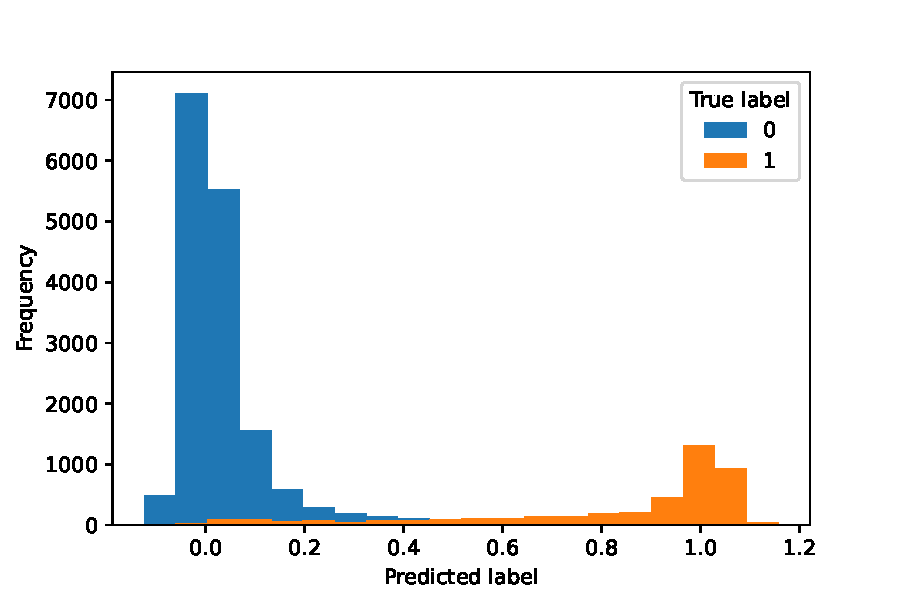
\includegraphics[width=\linewidth]{histogram-labels-bert-train.pdf}
        \subcaption{Predictions with \BertBase on the training set.}
        \label{subfig:bert_train}
    \end{subfigure}
    \hfill
    \begin{subfigure}{0.42\textwidth}
        \centering
        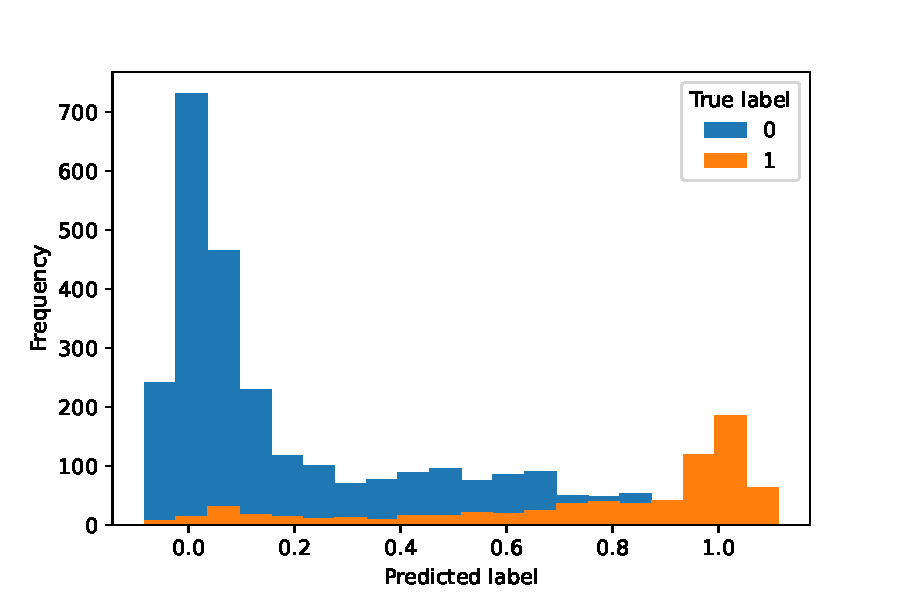
\includegraphics[width=\linewidth]{histogram-labels-bert-dev.pdf}
        \subcaption{Predictions with \BertBase on the validation set.}
        \label{subfig:bert_dev}
    \end{subfigure}
    \begin{subfigure}{0.42\textwidth}
        \centering
        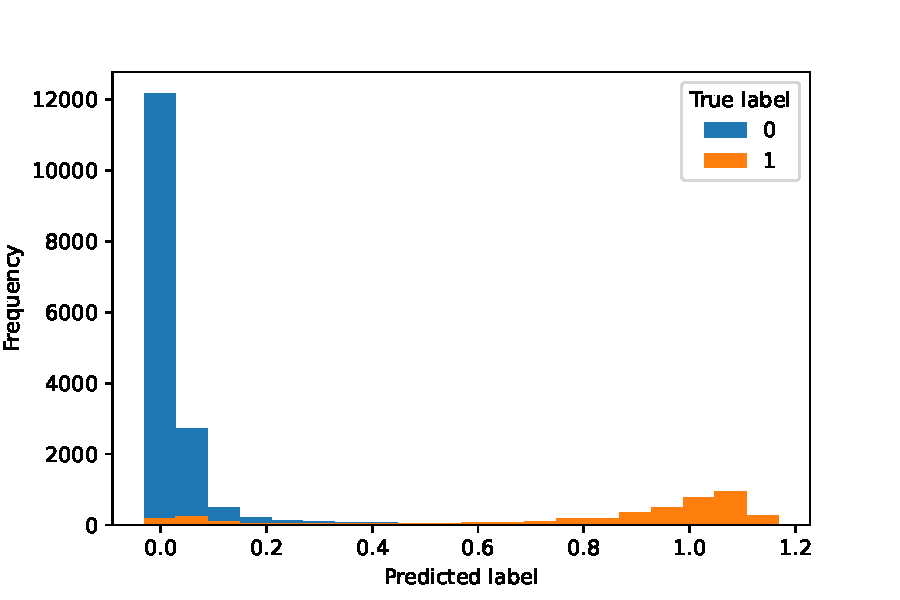
\includegraphics[width=\linewidth]{histogram-labels-roberta-train.pdf}
        \subcaption{Predictions with \RobertaBase on the training set.}
        \label{subfig:roberta_train}
    \end{subfigure}
    \hfill
    \begin{subfigure}{0.42\textwidth}
        \centering
        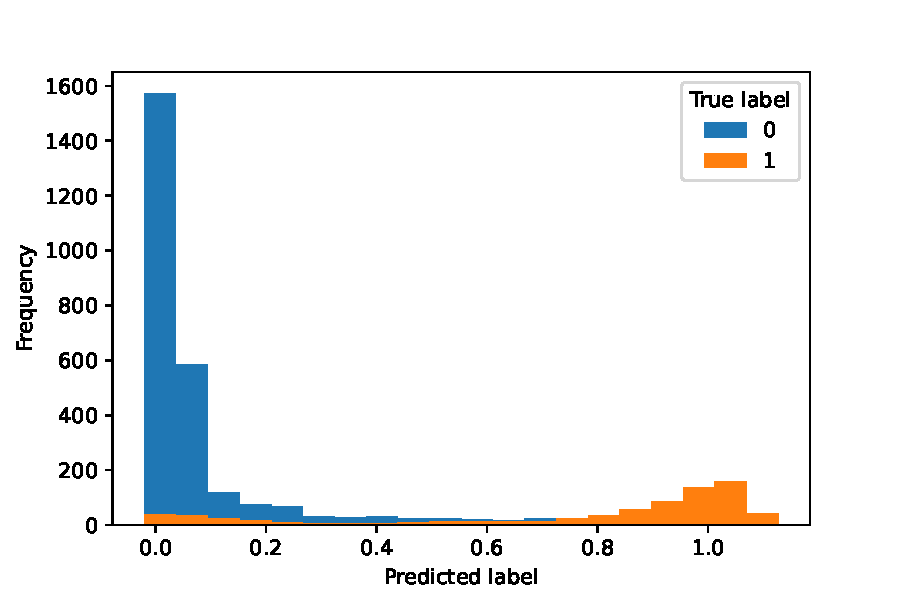
\includegraphics[width=\linewidth]{histogram-labels-roberta-dev.pdf}
        \subcaption{Predictions with \RobertaBase on the validation set.}
        \label{subfig:roberta_dev}
    \end{subfigure}
    \caption{Histograms of predicted labels on the training and validation sets for argument key point pairs with the \BertBase and \RobertaBase classifiers. For good classifiers, predicted labels should approximately equal the true label~(0~or~1).}
    \label{fig:frequency}
\end{figure*}
To find errors in the two trained matchers, \BertBase and \RobertaBase, in Figure~\ref{fig:frequency} we show histograms of predicted match scores with respect to ground-truth labels.
Both matchers classify most pairs correctly, which can be seen because the histogram spikes around~0 for the true no-match label and around~1 for the true match label.
We also observe that predictions on the training set are closer to the true label than on the development set for both \RobertaBase and \BertBase.
Even though we expect any machine-learned matcher to perform better on training data than on validation data, we see this as a room for improvement with better generalization.
We notice that in Figures~\ref{subfig:bert_train} and~\ref{subfig:roberta_train} both approaches predict non-matching argument key point pairs better than matching key points.
This effect is likely to occur because of the higher amount of non-matching pairs provided.
Most arguments match with only a few or even just a single key point.
But nonetheless each argument is compared to all other key points, hence the underlying data to learn from is imbalanced~\cite{BarandelaVSF2004}.
Though, experiments with using textual data augmentation to balance the dataset were unsuccessful.
Other approaches to balance the amount of matching and non-matching key points for each argument, e.g., oversampling or undersampling~\cite{Dietterich1995}, could resolve this issue.
We further identify, that for matching arguments and key points, predicted scores from \BertBase are spread a bit more than scores from \RobertaBase.

\begin{figure}
    \begin{tabularx}{\linewidth}{@{}lX@{}}
        Arg. & \texttt{School uniforms can be less comfortable than students' regular clothes.} \\
        KP & \texttt{School uniforms are expensive.} \\
        Pred. & \(0.48\) \\
    \end{tabularx}
    \caption{Argument and key point for the topic \texttt{We should abandon the use of school uniform} from the ArgKP dataset~\cite{Bar-HaimEFKLS2020}.}
    \label{example-4-162-6}
\end{figure}
In Figures~\ref{subfig:bert_dev} and~\ref{subfig:roberta_dev}, we observe that the \BertBase matcher falsely classifies certain non-matching and matching pairs. The argument key point pair shown in Figure~\ref{example-4-162-6} seems to be particularily hard to classify.
One reason we identify is that this argument has no matching key points given in the training dataset.
Hence it is plausible that the \BertBase has not learned well how to classify matches for that type of argument, and therefore predicts a label of~\(0.48\).

\begin{figure}
    \begin{tabularx}{\linewidth}{@{}p{2em}X@{}}
        Arg. & \texttt{affirmative action can lead to people who are less qualified getting positions they would otherwise not be able to achieve} \\
        Arg. & \texttt{affirmative action discriminates the majority, preventing skilled workers from gaining employment over someone less qualified but considered to be a member of a protected minority group.}
    \end{tabularx}
    \caption{Matching arguments to the key point \texttt{Affirmative action reduces quality.} that are falsely classified as non-matching by the \BertBase matcher.}
    \label{example-5-110-113}
\end{figure}
\begin{figure}
    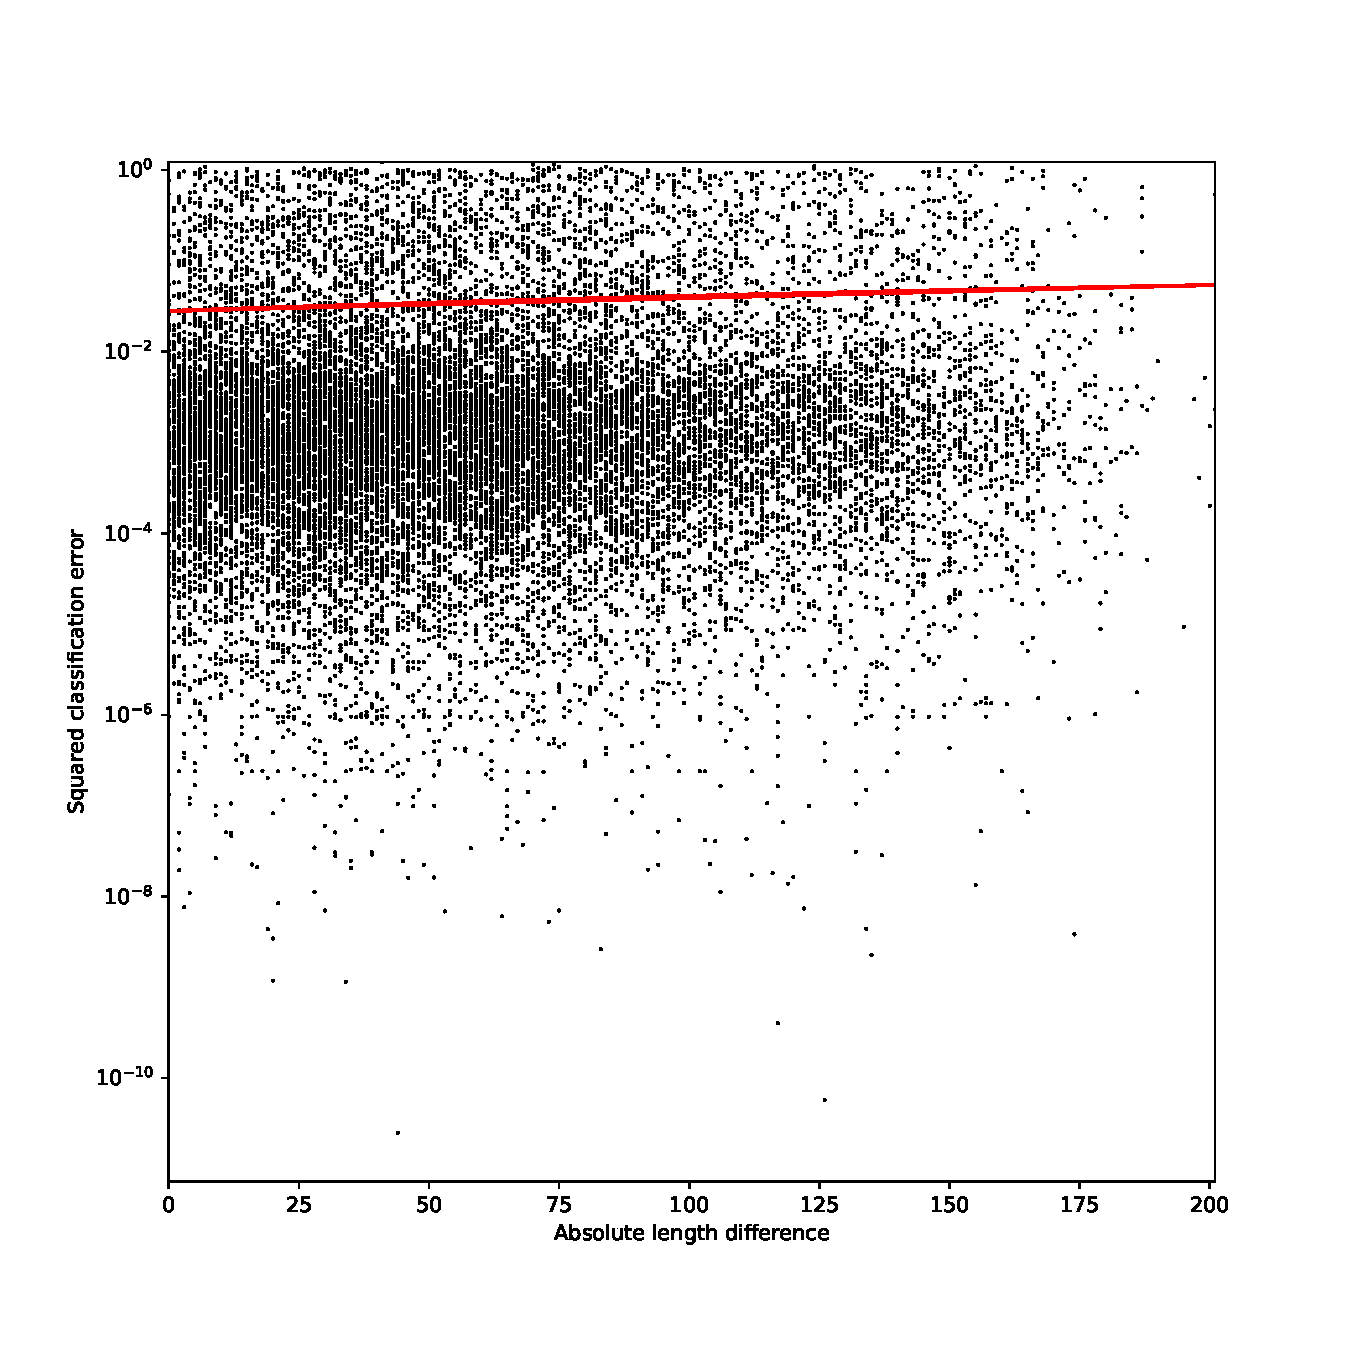
\includegraphics[width=\linewidth]{classification-error-length-difference-bert-train.pdf}
    \caption{Squared classification error and absolute length difference between each argument and key point pair from the validation set with the \BertBase matcher. The red line indicates the least squares polynomial fit.}
    \label{classification-error-length}
\end{figure}
The same \BertBase matcher falsely predicts some argument key point pairs as non-matching.
For example, it seems to be very difficult to predict matches for the key point \texttt{Affirmative action reduces quality.} from the topic \texttt{We should end affirmative action}, as shown in Figure~\ref{example-5-110-113}. These two arguments are longer than most arguments %\todo{from that topic?}
and especially longer than the key point.
It might be more challenging to reduce such longer arguments, containing more complex information, to very compact key points.
We confirm that observation by comparing the squared classification error with respect to the absolute difference between argument and key point lengths.
Figure~\ref{classification-error-length} shows a tendency of higher error with the \BertBase when the length difference between the argument and key point is large.
Comparable results can be observed for the \Roberta model.
We therefore identify length difference as a second general problem for both approaches.

\section{Conclusion and Future Work}\label{conclusion}

We approach the practical problem of matching arguments to summarizing, short key points.
Although our token overlap baseline approach is very simple, it achieves a mean average precision of up to~0.575 on 
the test set, nearly double the score of a random matcher. 
The baseline approach is straightforward to implement but cannot eliminate the problem of context understanding. 
\RobertaBase and \BertBase have achieved good performance, because they can overcome the context understanding challenge. 
Our fine-tuned \RobertaBase model also performed better than \BertBase in this task and scores a mean average 
precision of up to~0.967.
With strict ground truth labels it achieves a mean average precision score of~0.913 on the test set, which is the best 
score of the participating teams in the shared task.
This again shows the importance of architecture, training objectives, and hyperparameter selection.

\subsection{Future Work}

We identify two main issues with the language model approach:
First, both the \BertBase and \RobertaBase model cannot adequately match arguments that have no matching key point in the training set.
This could maybe be improved by resampling data or transfer learning.
Second, both models tend to classify argument key point pairs worse if the argument and key point largely differ in length.
We see this as a potential to combine the transformer matchers with the token overlap baseline because for longer arguments 
it can be more likely that all tokens from the key point occur in it.
Another possible improvement are recent improvements in language models~\cite{Sun2021WFDPSLCZLLWGLSSLOYTWW}.
If a language model is even more robust than, for example, \Roberta, we expect a fine-tuned matcher to outperform 
the \RobertaBase matcher as well.


% Entries for the entire Anthology, followed by custom entries
\bibliography{anthology,custom}
\bibliographystyle{acl_natbib}

\appendix

% \appendix
% \section{Appendix}

% {\color{red}
%     \subsection{ToDo's}
%     \begin{itemize}
%         \item key-point vs. key point vs. keypoint
%         \item pretrained vs. pre-trained
%         \item comma separator: \verb|.|
%         \item thousands separator: \verb|\,|
%     \end{itemize}
% }


\todo{Consistently use normal case or Title Case for fields of research.}

\end{document}
